\documentclass[11pt]{article}
\usepackage[textwidth=18.0cm, textheight=23.0cm, top=2.0cm]{geometry}
\usepackage{pst-all}
\usepackage{amssymb}
\usepackage{tikz}
\usepackage{underscore}\begin{document}
\pagestyle{empty}


ClassName: \underline{\textbf{Class_05.2bp-18}}
\par
BinSize: \underline{\textbf{100 × 100}}
\par
ReduceSize: \underline{\textbf{100 × 100}}
\par
TypeNum: \underline{\textbf{40}}
\par
Num: \underline{\textbf{40}}
\par
OutS: \underline{\textbf{100000}}
\par
InS: \underline{\textbf{83980}}
\par
Rate: \underline{\textbf{0.840}}
\par
UB: \underline{\textbf{10}}
\par
LB0: \underline{\textbf{9}}
\par
LB: \underline{\textbf{10}}
\par
LBWithCut: \underline{\textbf{10}}
\par
NodeCut: \underline{\textbf{0}}
\par
ExtendedNodeCnt: \underline{\textbf{1}}
\par
GenNodeCnt: \underline{\textbf{1}}
\par
PrimalNode: \underline{\textbf{0}}
\par
ColumnCount: \underline{\textbf{102}}
\par
TotalCutCount: \underline{\textbf{0}}
\par
RootCutCount: \underline{\textbf{0}}
\par
LPSolverCnt: \underline{\textbf{93}}
\par
PricingSolverCnt: \underline{\textbf{93}}
\par
BranchAndBoundNum: \underline{\textbf{1}}
\par
isOpt: \underline{\textbf{true}}
\par
TimeOnInitSolution: \underline{\textbf{0.030 s}}
\par
TimeOnPrimal: \underline{\textbf{0.000 s}}
\par
TimeOnPricing: \underline{\textbf{95.625 s}}
\par
TimeOnRmp: \underline{\textbf{0.098 s}}
\par
TotalTime: \underline{\textbf{95.867 s}}
\par
\newpage


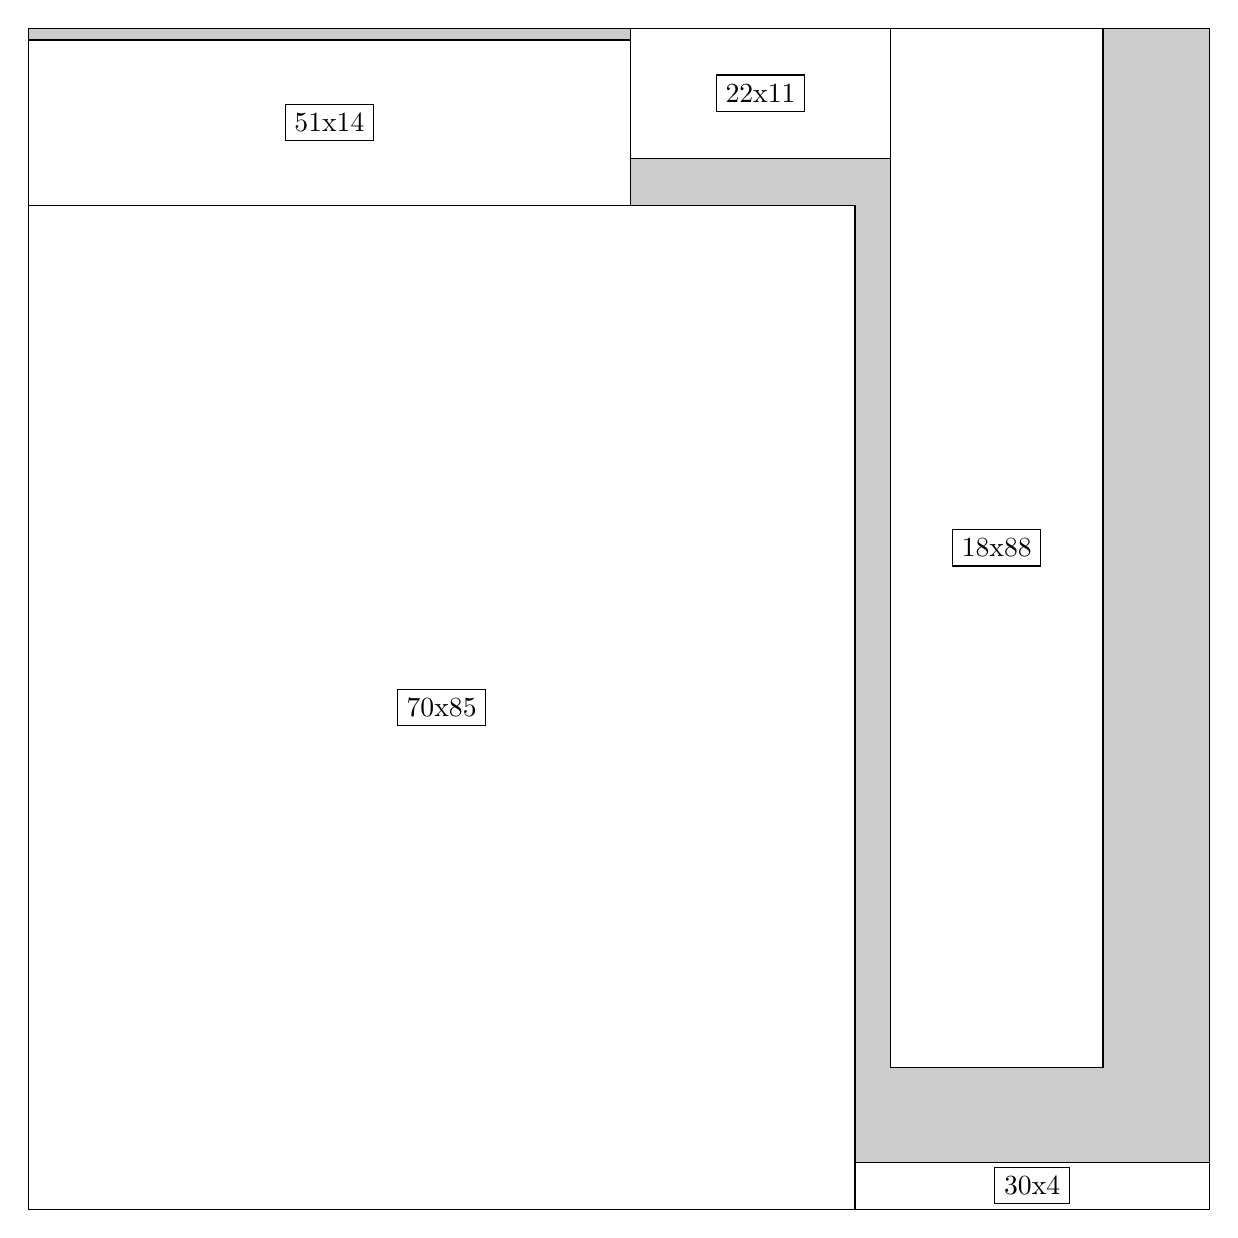
\begin{tikzpicture}[shorten >=1pt,scale=1.0,every node/.style={scale=1.0},->]
\tikzstyle{vertex}=[circle,fill=black!25,minimum size=14pt,inner sep=0pt]
\filldraw[fill=gray!40!white, draw=black] (0,0) rectangle (15.0,15.0);
\foreach \name/\x/\y/\w/\h in {70x85/0.0/0.0/10.5/12.75,18x88/10.95/1.7999999999999998/2.6999999999999997/13.2,51x14/0.0/12.75/7.6499999999999995/2.1,22x11/7.6499999999999995/13.35/3.3/1.65,30x4/10.5/0.0/4.5/0.6}
\filldraw[fill=white!40!white, draw=black] (\x,\y) rectangle node[draw] (\name) {\name} ++(\w,\h);
\end{tikzpicture}


w =70 , h =85 , x =0 , y =0 , v =5950
\par
w =18 , h =88 , x =73 , y =12 , v =1584
\par
w =51 , h =14 , x =0 , y =85 , v =714
\par
w =22 , h =11 , x =51 , y =89 , v =242
\par
w =30 , h =4 , x =70 , y =0 , v =120
\par
\newpage


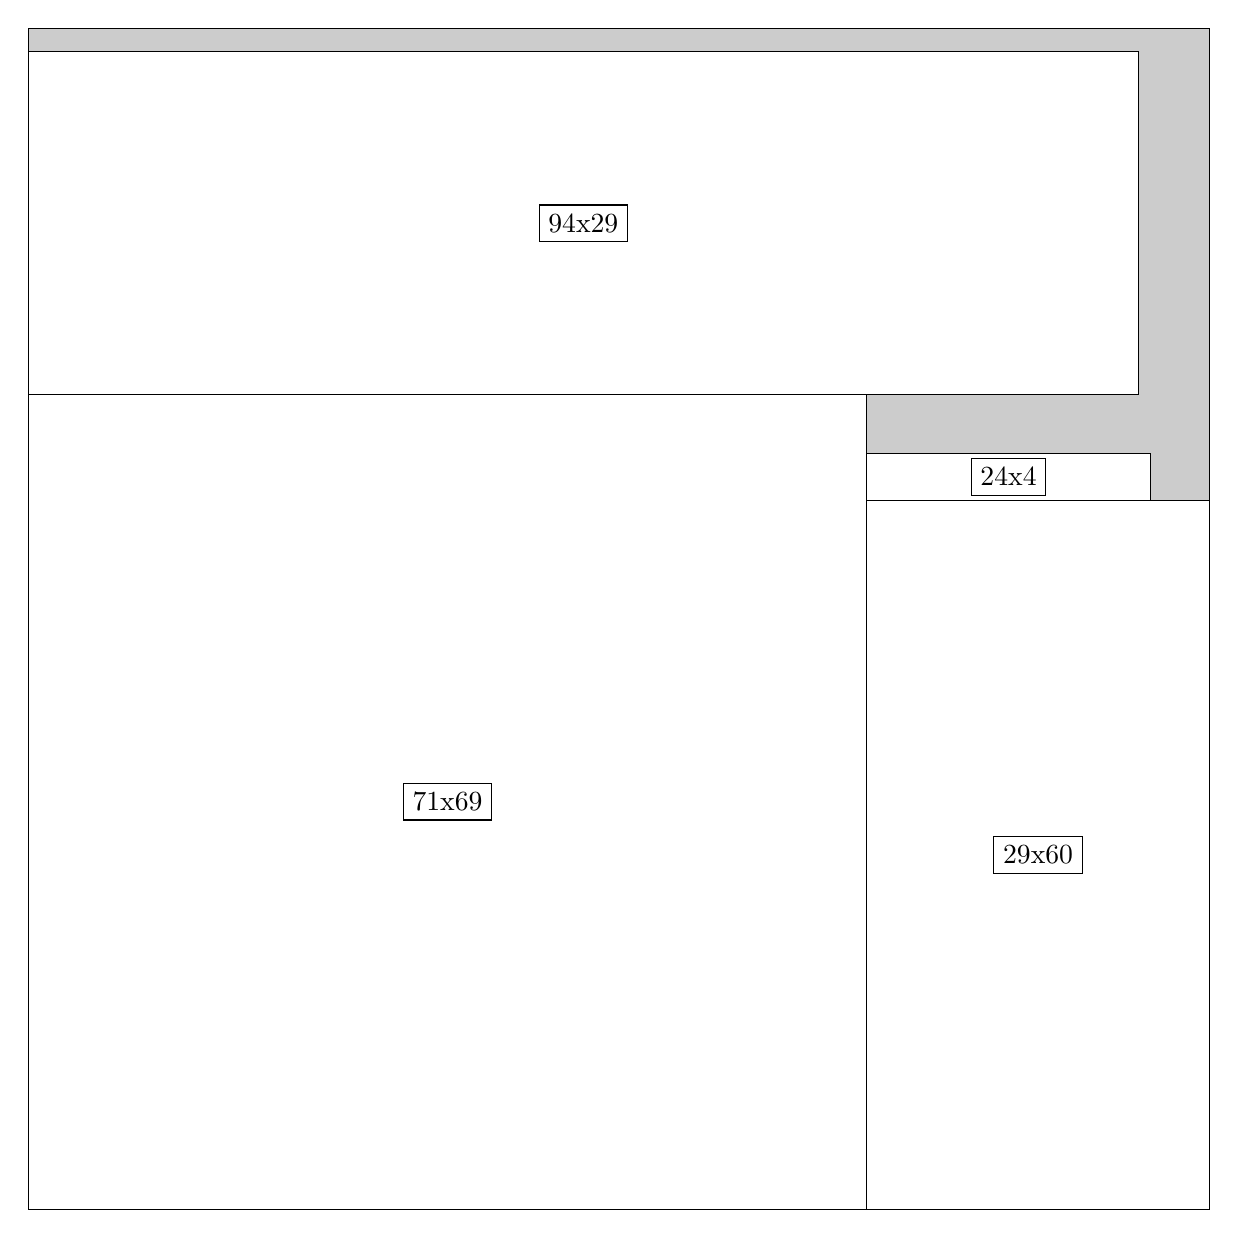
\begin{tikzpicture}[shorten >=1pt,scale=1.0,every node/.style={scale=1.0},->]
\tikzstyle{vertex}=[circle,fill=black!25,minimum size=14pt,inner sep=0pt]
\filldraw[fill=gray!40!white, draw=black] (0,0) rectangle (15.0,15.0);
\foreach \name/\x/\y/\w/\h in {71x69/0.0/0.0/10.65/10.35,94x29/0.0/10.35/14.1/4.35,29x60/10.65/0.0/4.35/9.0,24x4/10.65/9.0/3.5999999999999996/0.6}
\filldraw[fill=white!40!white, draw=black] (\x,\y) rectangle node[draw] (\name) {\name} ++(\w,\h);
\end{tikzpicture}


w =71 , h =69 , x =0 , y =0 , v =4899
\par
w =94 , h =29 , x =0 , y =69 , v =2726
\par
w =29 , h =60 , x =71 , y =0 , v =1740
\par
w =24 , h =4 , x =71 , y =60 , v =96
\par
\newpage


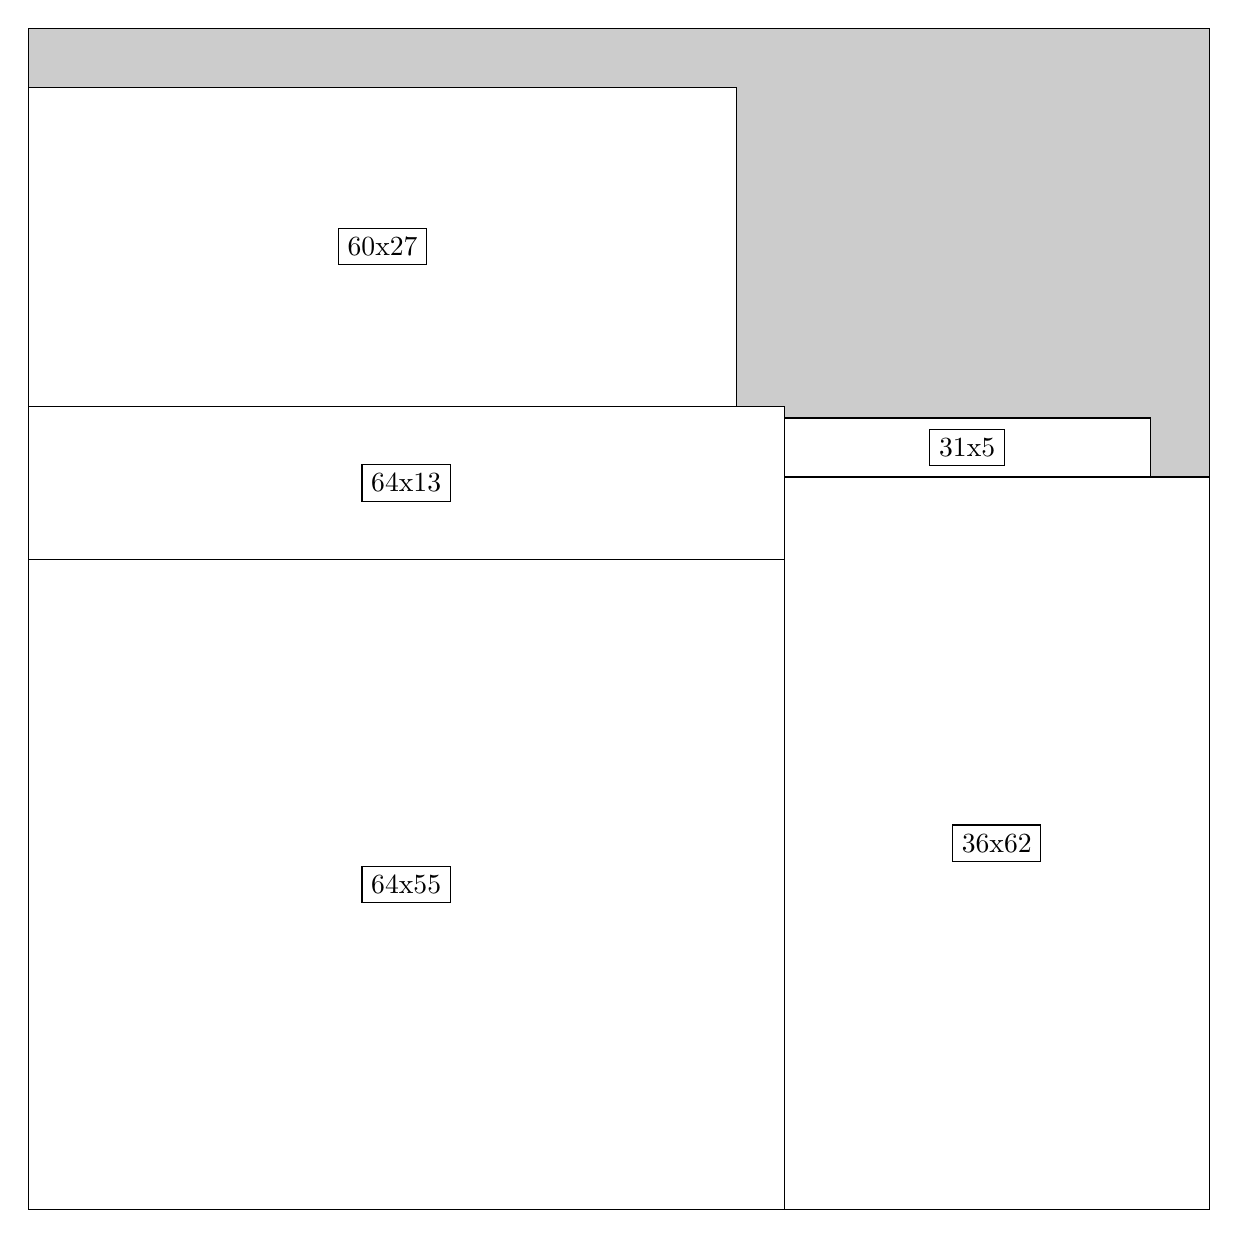
\begin{tikzpicture}[shorten >=1pt,scale=1.0,every node/.style={scale=1.0},->]
\tikzstyle{vertex}=[circle,fill=black!25,minimum size=14pt,inner sep=0pt]
\filldraw[fill=gray!40!white, draw=black] (0,0) rectangle (15.0,15.0);
\foreach \name/\x/\y/\w/\h in {64x55/0.0/0.0/9.6/8.25,36x62/9.6/0.0/5.3999999999999995/9.299999999999999,60x27/0.0/10.2/9.0/4.05,64x13/0.0/8.25/9.6/1.95,31x5/9.6/9.299999999999999/4.6499999999999995/0.75}
\filldraw[fill=white!40!white, draw=black] (\x,\y) rectangle node[draw] (\name) {\name} ++(\w,\h);
\end{tikzpicture}


w =64 , h =55 , x =0 , y =0 , v =3520
\par
w =36 , h =62 , x =64 , y =0 , v =2232
\par
w =60 , h =27 , x =0 , y =68 , v =1620
\par
w =64 , h =13 , x =0 , y =55 , v =832
\par
w =31 , h =5 , x =64 , y =62 , v =155
\par
\newpage


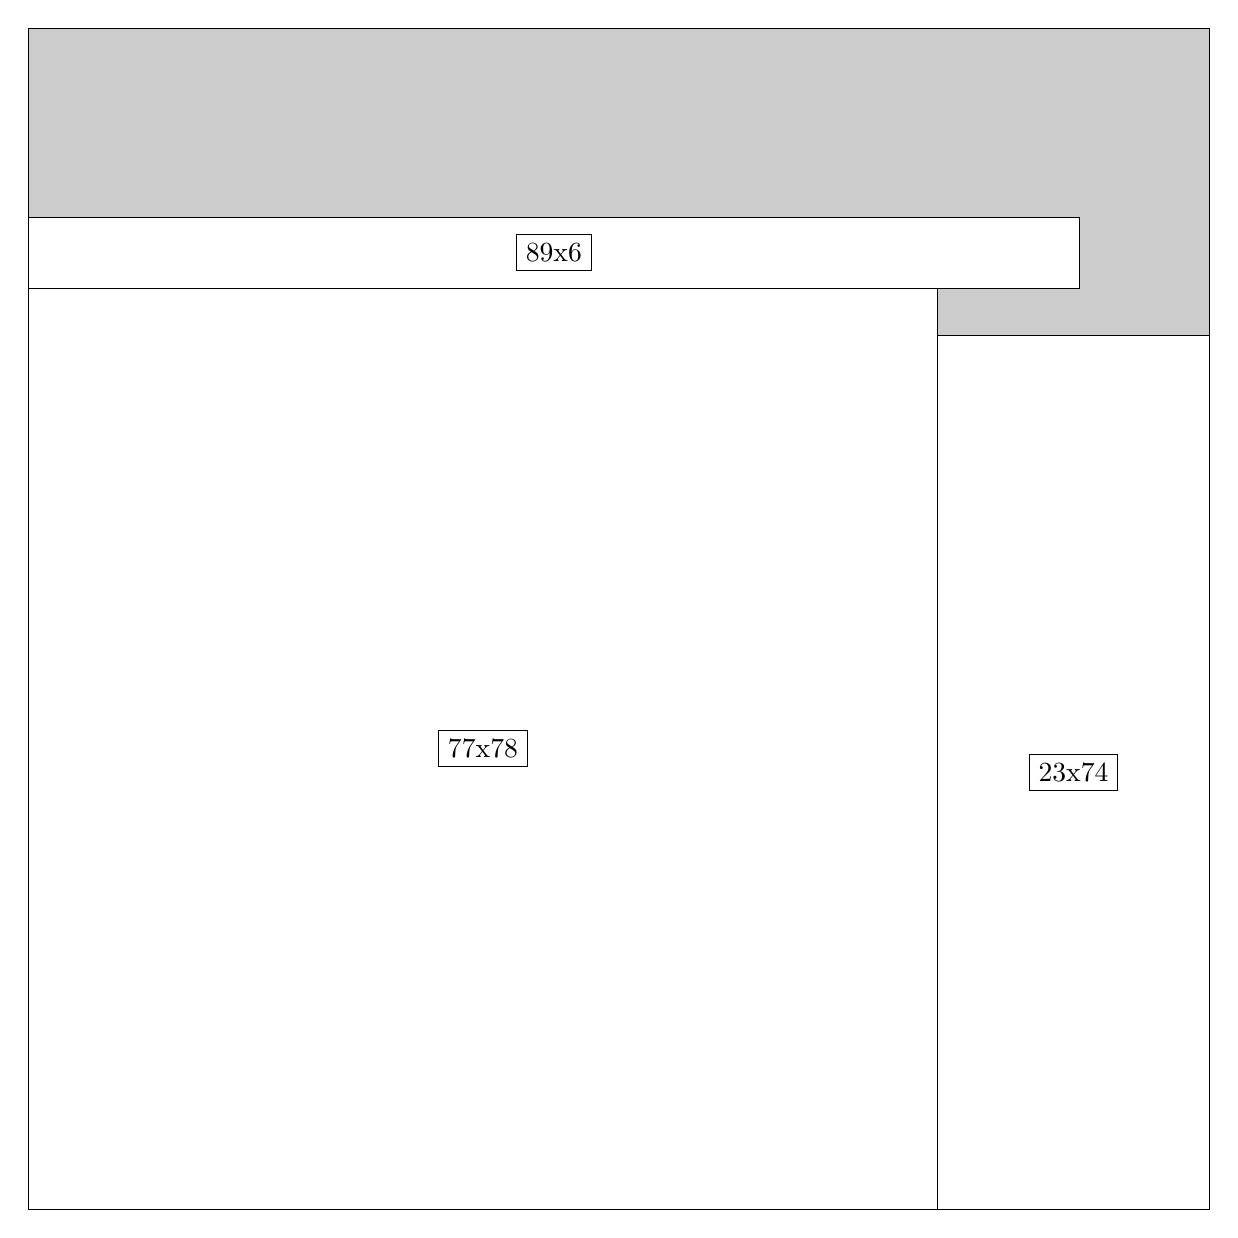
\begin{tikzpicture}[shorten >=1pt,scale=1.0,every node/.style={scale=1.0},->]
\tikzstyle{vertex}=[circle,fill=black!25,minimum size=14pt,inner sep=0pt]
\filldraw[fill=gray!40!white, draw=black] (0,0) rectangle (15.0,15.0);
\foreach \name/\x/\y/\w/\h in {23x74/11.549999999999999/0.0/3.4499999999999997/11.1,77x78/0.0/0.0/11.549999999999999/11.7,89x6/0.0/11.7/13.35/0.8999999999999999}
\filldraw[fill=white!40!white, draw=black] (\x,\y) rectangle node[draw] (\name) {\name} ++(\w,\h);
\end{tikzpicture}


w =23 , h =74 , x =77 , y =0 , v =1702
\par
w =77 , h =78 , x =0 , y =0 , v =6006
\par
w =89 , h =6 , x =0 , y =78 , v =534
\par
\newpage


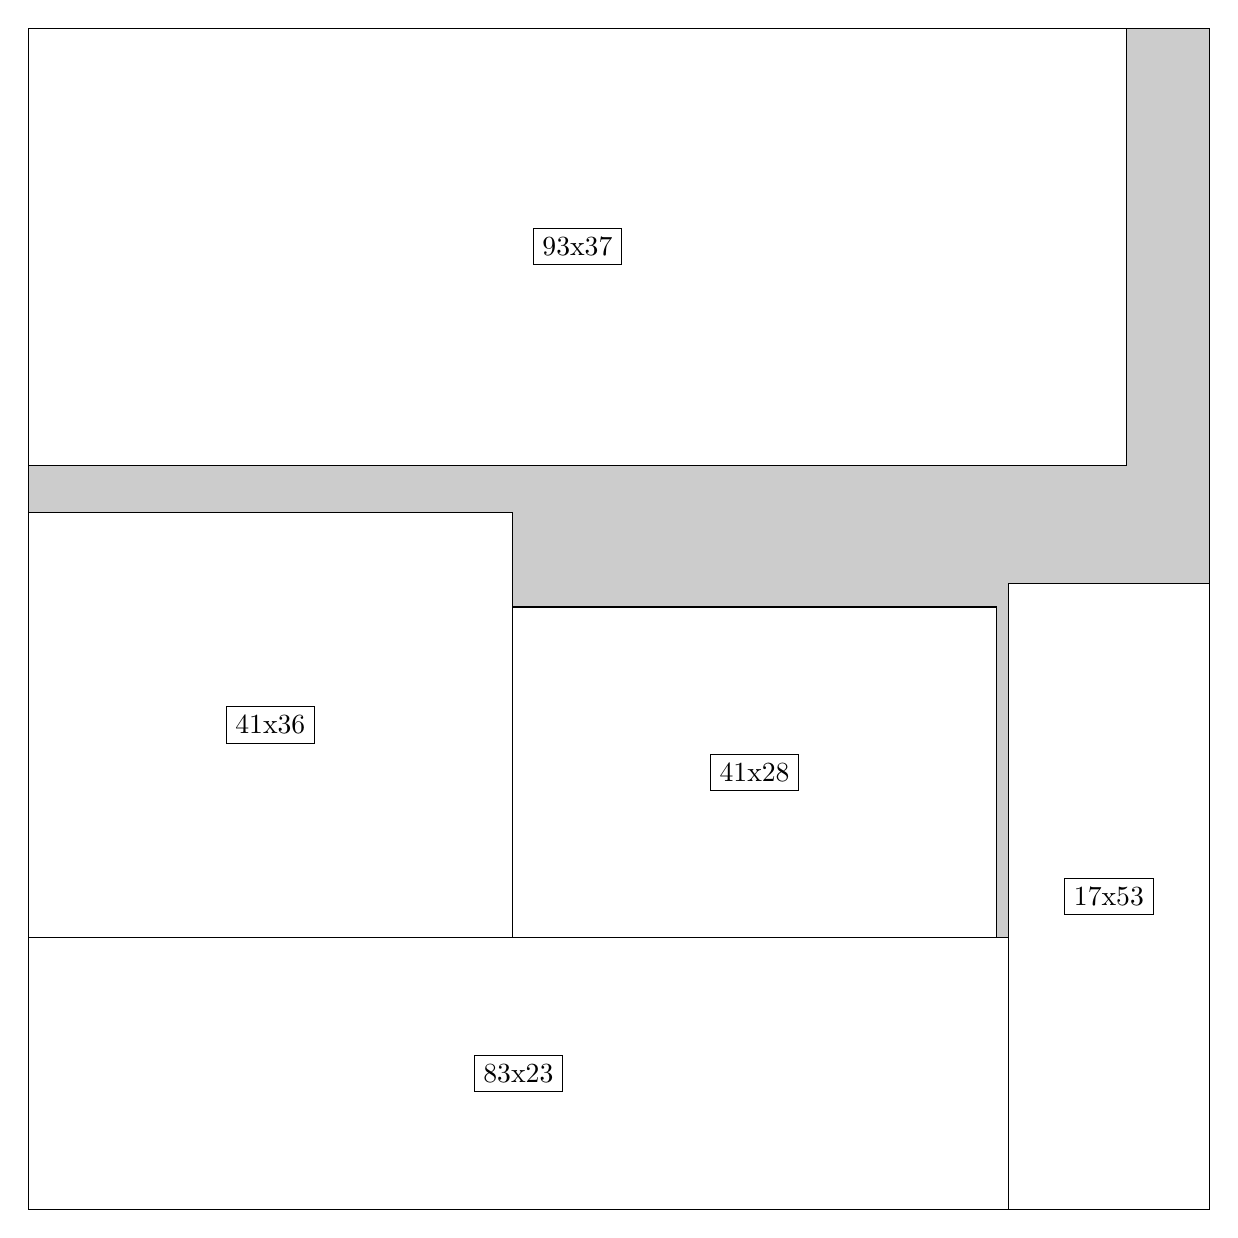
\begin{tikzpicture}[shorten >=1pt,scale=1.0,every node/.style={scale=1.0},->]
\tikzstyle{vertex}=[circle,fill=black!25,minimum size=14pt,inner sep=0pt]
\filldraw[fill=gray!40!white, draw=black] (0,0) rectangle (15.0,15.0);
\foreach \name/\x/\y/\w/\h in {83x23/0.0/0.0/12.45/3.4499999999999997,93x37/0.0/9.45/13.95/5.55,41x36/0.0/3.4499999999999997/6.1499999999999995/5.3999999999999995,41x28/6.1499999999999995/3.4499999999999997/6.1499999999999995/4.2,17x53/12.45/0.0/2.55/7.949999999999999}
\filldraw[fill=white!40!white, draw=black] (\x,\y) rectangle node[draw] (\name) {\name} ++(\w,\h);
\end{tikzpicture}


w =83 , h =23 , x =0 , y =0 , v =1909
\par
w =93 , h =37 , x =0 , y =63 , v =3441
\par
w =41 , h =36 , x =0 , y =23 , v =1476
\par
w =41 , h =28 , x =41 , y =23 , v =1148
\par
w =17 , h =53 , x =83 , y =0 , v =901
\par
\newpage


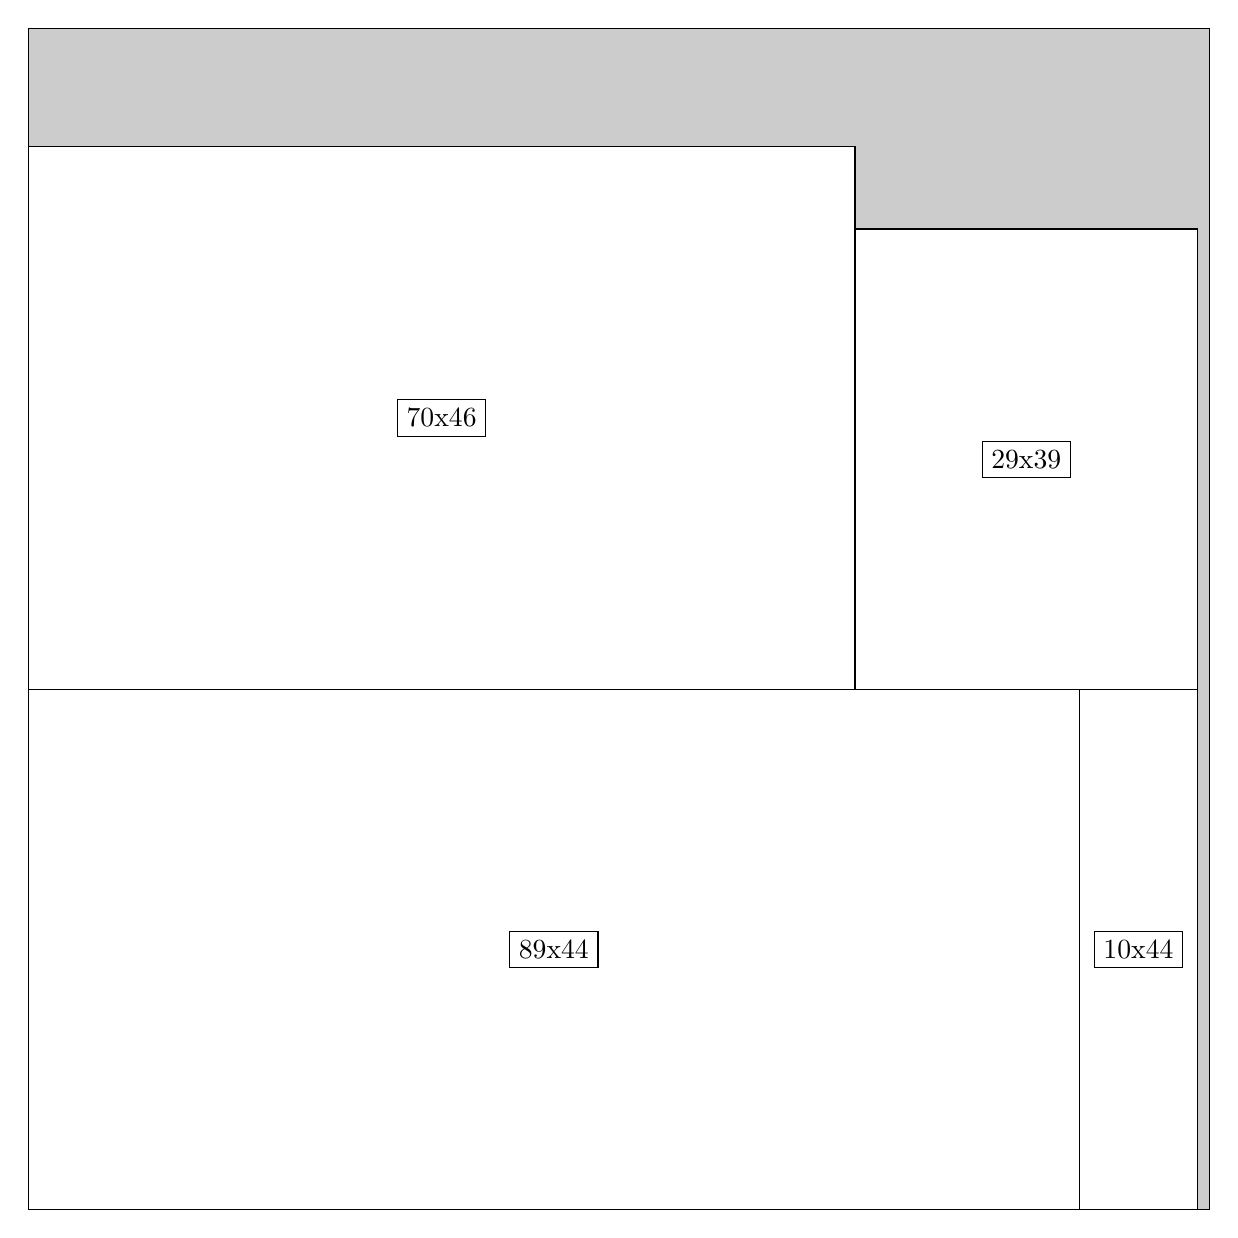
\begin{tikzpicture}[shorten >=1pt,scale=1.0,every node/.style={scale=1.0},->]
\tikzstyle{vertex}=[circle,fill=black!25,minimum size=14pt,inner sep=0pt]
\filldraw[fill=gray!40!white, draw=black] (0,0) rectangle (15.0,15.0);
\foreach \name/\x/\y/\w/\h in {89x44/0.0/0.0/13.35/6.6,70x46/0.0/6.6/10.5/6.8999999999999995,29x39/10.5/6.6/4.35/5.85,10x44/13.35/0.0/1.5/6.6}
\filldraw[fill=white!40!white, draw=black] (\x,\y) rectangle node[draw] (\name) {\name} ++(\w,\h);
\end{tikzpicture}


w =89 , h =44 , x =0 , y =0 , v =3916
\par
w =70 , h =46 , x =0 , y =44 , v =3220
\par
w =29 , h =39 , x =70 , y =44 , v =1131
\par
w =10 , h =44 , x =89 , y =0 , v =440
\par
\newpage


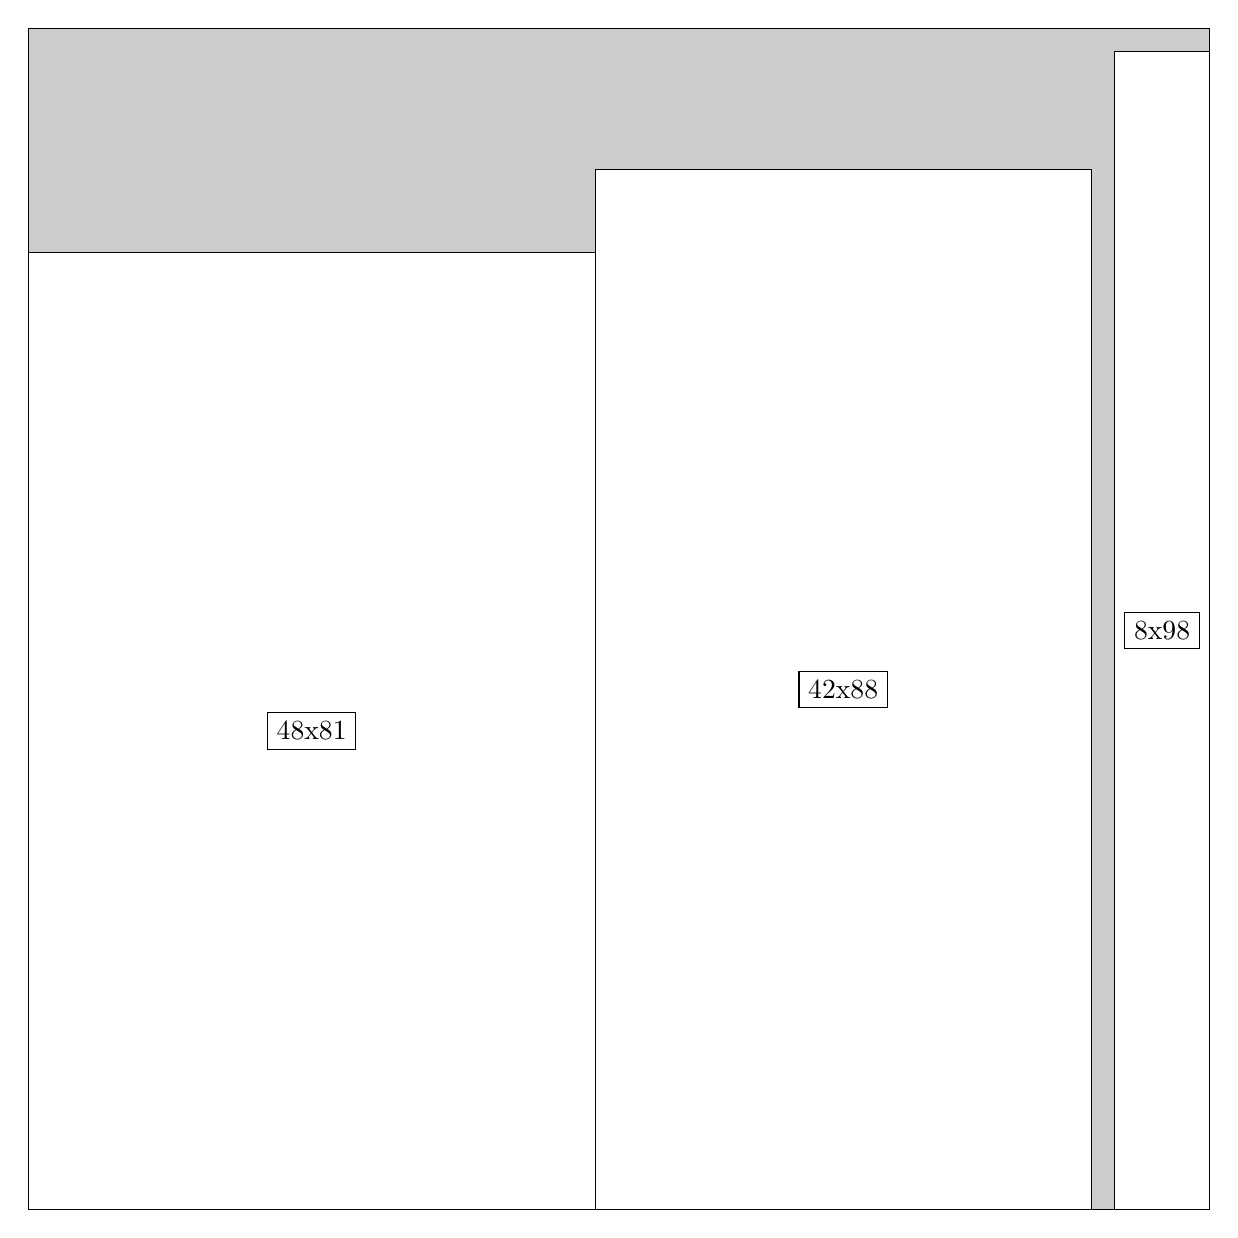
\begin{tikzpicture}[shorten >=1pt,scale=1.0,every node/.style={scale=1.0},->]
\tikzstyle{vertex}=[circle,fill=black!25,minimum size=14pt,inner sep=0pt]
\filldraw[fill=gray!40!white, draw=black] (0,0) rectangle (15.0,15.0);
\foreach \name/\x/\y/\w/\h in {48x81/0.0/0.0/7.199999999999999/12.15,42x88/7.199999999999999/0.0/6.3/13.2,8x98/13.799999999999999/0.0/1.2/14.7}
\filldraw[fill=white!40!white, draw=black] (\x,\y) rectangle node[draw] (\name) {\name} ++(\w,\h);
\end{tikzpicture}


w =48 , h =81 , x =0 , y =0 , v =3888
\par
w =42 , h =88 , x =48 , y =0 , v =3696
\par
w =8 , h =98 , x =92 , y =0 , v =784
\par
\newpage


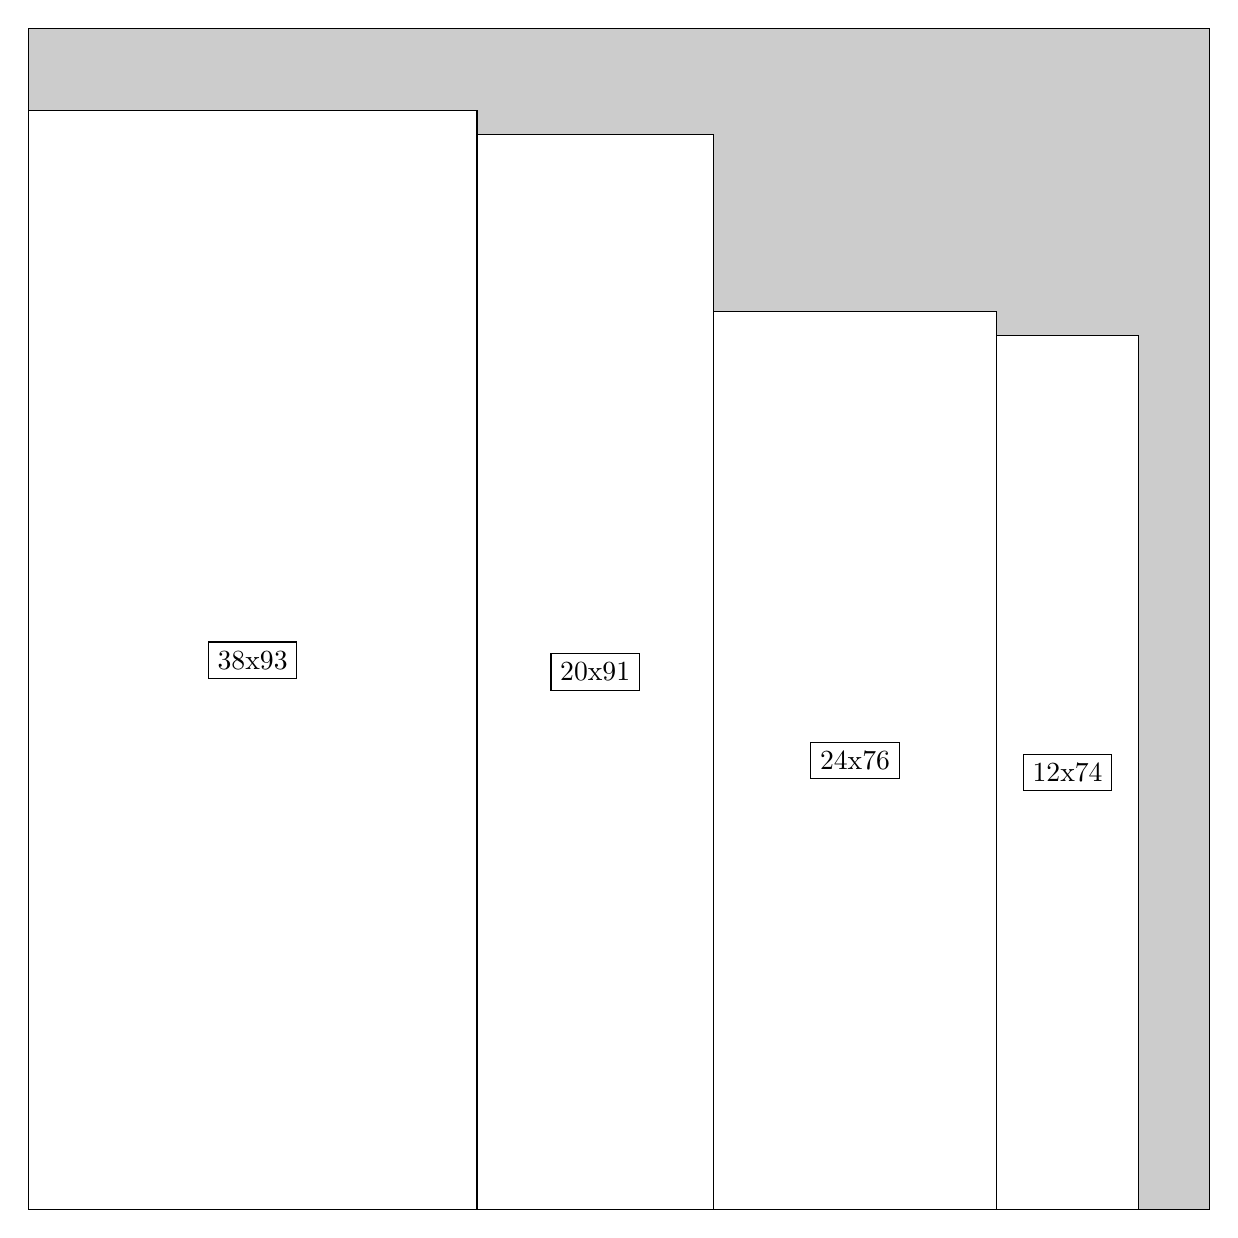
\begin{tikzpicture}[shorten >=1pt,scale=1.0,every node/.style={scale=1.0},->]
\tikzstyle{vertex}=[circle,fill=black!25,minimum size=14pt,inner sep=0pt]
\filldraw[fill=gray!40!white, draw=black] (0,0) rectangle (15.0,15.0);
\foreach \name/\x/\y/\w/\h in {38x93/0.0/0.0/5.7/13.95,24x76/8.7/0.0/3.5999999999999996/11.4,20x91/5.7/0.0/3.0/13.65,12x74/12.299999999999999/0.0/1.7999999999999998/11.1}
\filldraw[fill=white!40!white, draw=black] (\x,\y) rectangle node[draw] (\name) {\name} ++(\w,\h);
\end{tikzpicture}


w =38 , h =93 , x =0 , y =0 , v =3534
\par
w =24 , h =76 , x =58 , y =0 , v =1824
\par
w =20 , h =91 , x =38 , y =0 , v =1820
\par
w =12 , h =74 , x =82 , y =0 , v =888
\par
\newpage


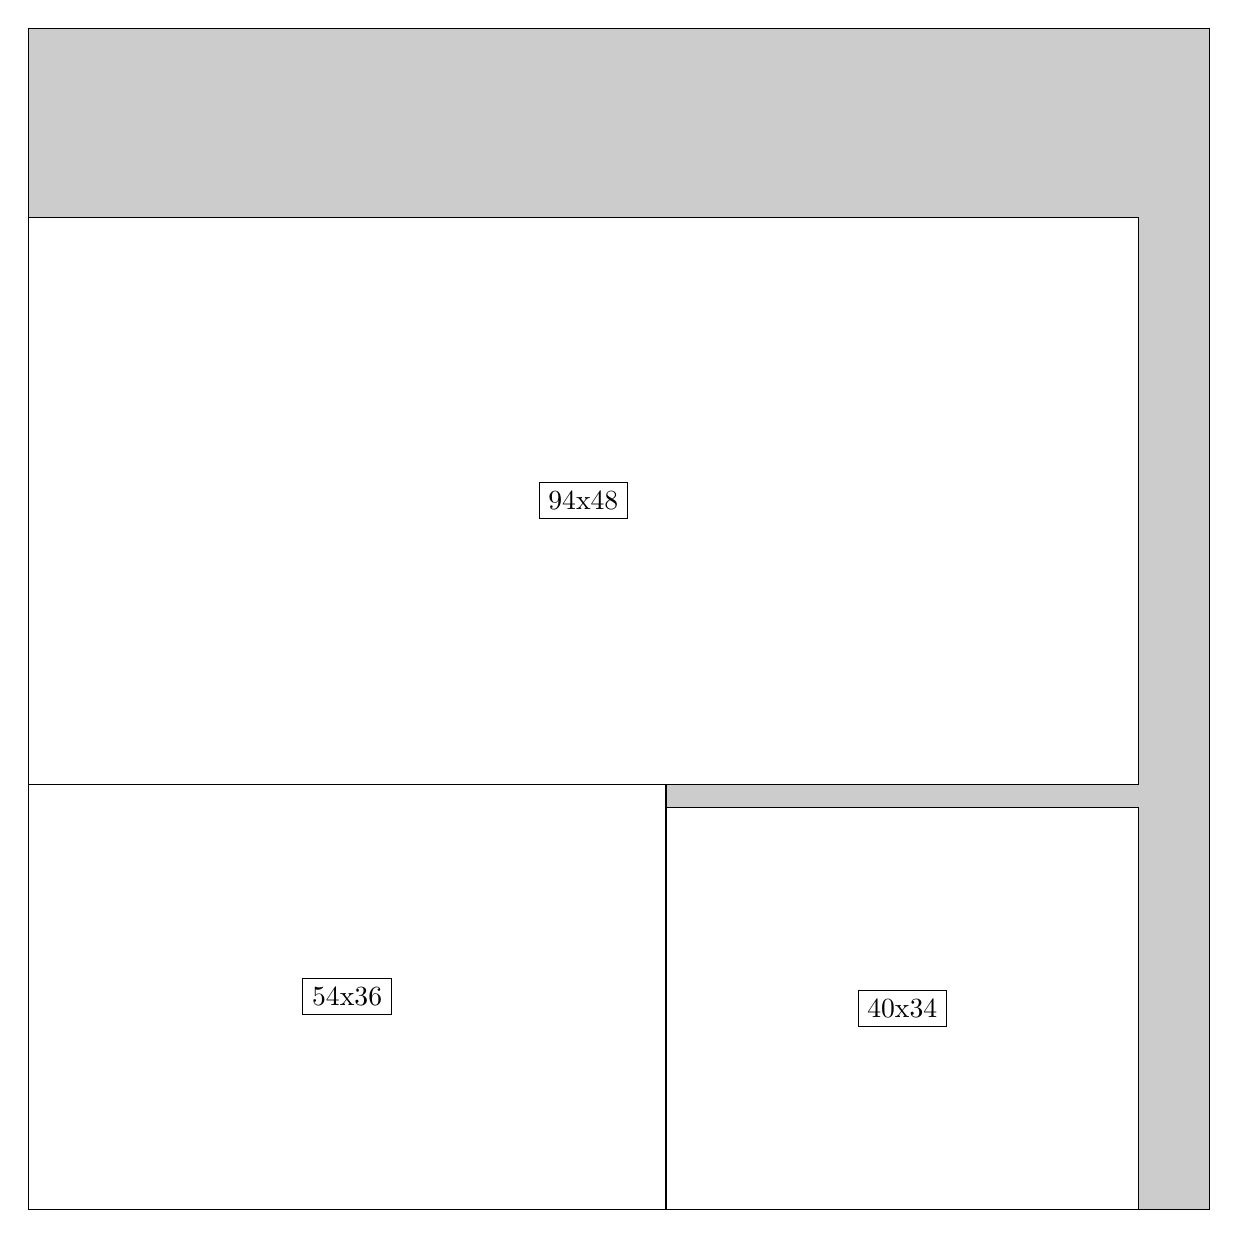
\begin{tikzpicture}[shorten >=1pt,scale=1.0,every node/.style={scale=1.0},->]
\tikzstyle{vertex}=[circle,fill=black!25,minimum size=14pt,inner sep=0pt]
\filldraw[fill=gray!40!white, draw=black] (0,0) rectangle (15.0,15.0);
\foreach \name/\x/\y/\w/\h in {94x48/0.0/5.3999999999999995/14.1/7.199999999999999,54x36/0.0/0.0/8.1/5.3999999999999995,40x34/8.1/0.0/6.0/5.1}
\filldraw[fill=white!40!white, draw=black] (\x,\y) rectangle node[draw] (\name) {\name} ++(\w,\h);
\end{tikzpicture}


w =94 , h =48 , x =0 , y =36 , v =4512
\par
w =54 , h =36 , x =0 , y =0 , v =1944
\par
w =40 , h =34 , x =54 , y =0 , v =1360
\par
\newpage


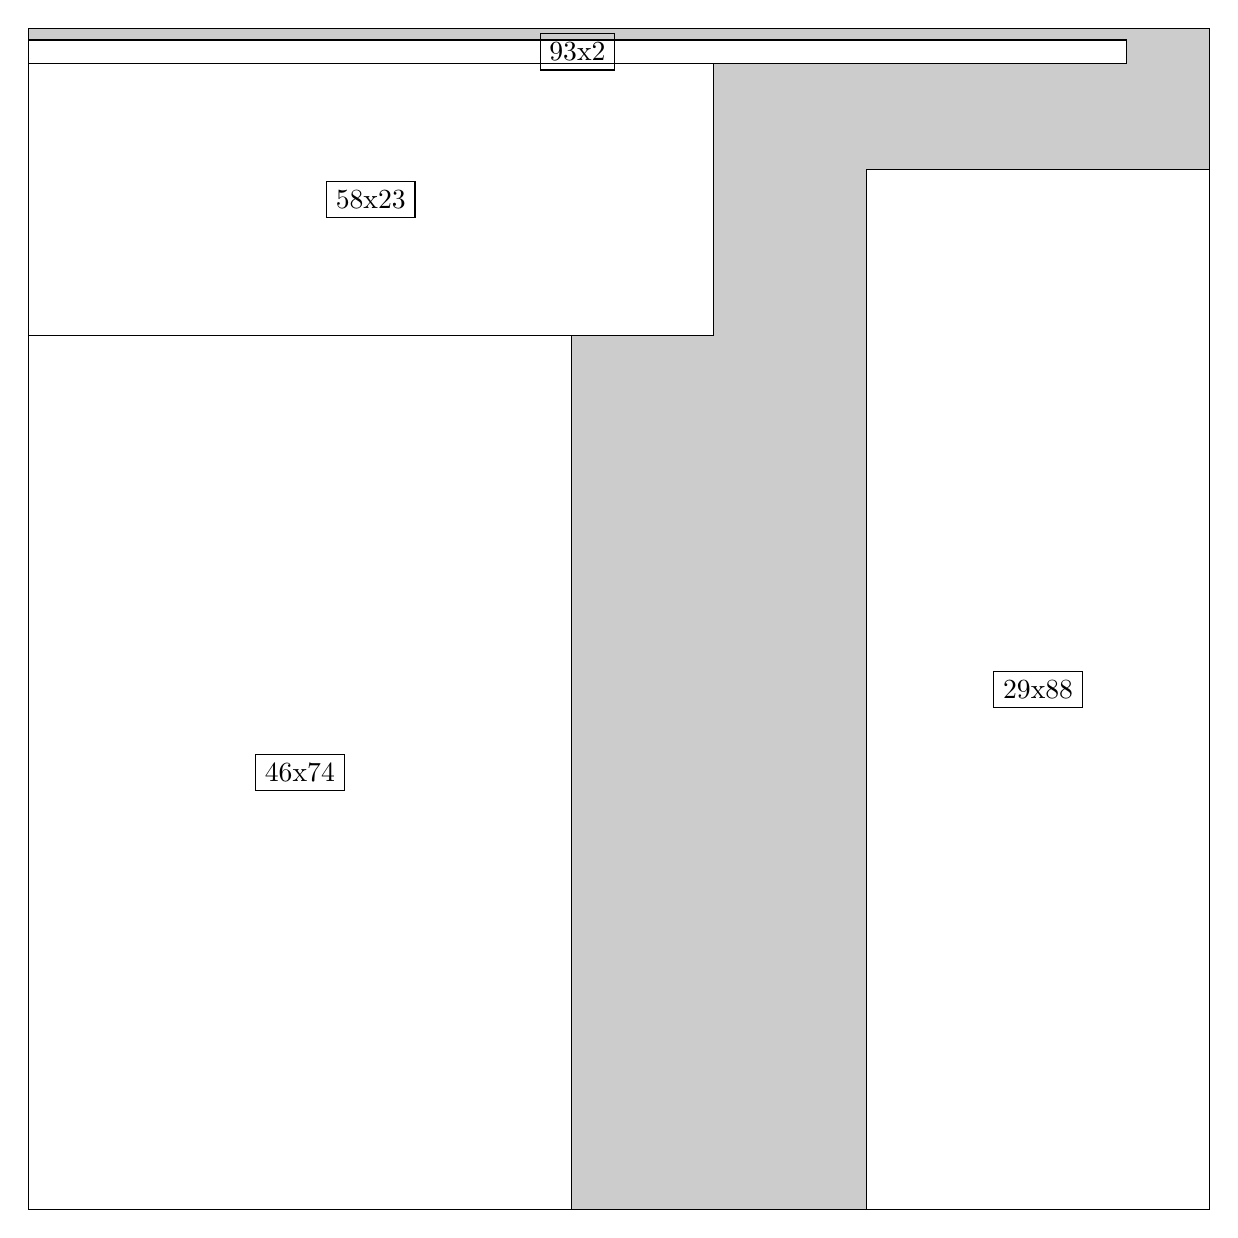
\begin{tikzpicture}[shorten >=1pt,scale=1.0,every node/.style={scale=1.0},->]
\tikzstyle{vertex}=[circle,fill=black!25,minimum size=14pt,inner sep=0pt]
\filldraw[fill=gray!40!white, draw=black] (0,0) rectangle (15.0,15.0);
\foreach \name/\x/\y/\w/\h in {46x74/0.0/0.0/6.8999999999999995/11.1,29x88/10.65/0.0/4.35/13.2,58x23/0.0/11.1/8.7/3.4499999999999997,93x2/0.0/14.549999999999999/13.95/0.3}
\filldraw[fill=white!40!white, draw=black] (\x,\y) rectangle node[draw] (\name) {\name} ++(\w,\h);
\end{tikzpicture}


w =46 , h =74 , x =0 , y =0 , v =3404
\par
w =29 , h =88 , x =71 , y =0 , v =2552
\par
w =58 , h =23 , x =0 , y =74 , v =1334
\par
w =93 , h =2 , x =0 , y =97 , v =186
\par
\newpage


\end{document}